% !TEX encoding = UTF-8
\documentclass[UTF8]{ctexart}

\usepackage[utf8]{inputenc}
\usepackage{graphicx}
\usepackage{geometry}
\geometry{a4paper}
\geometry{left=2.5cm,right=2.5cm,top=2.8cm,bottom=1.3cm}

\usepackage{booktabs}
\usepackage{array}
\usepackage{paralist}
\usepackage{verbatim}
\usepackage{subfig}
\usepackage{amsmath}
\usepackage{mathtools}
\usepackage{listings}
\usepackage[table]{xcolor}
\usepackage{lastpage}
\usepackage{url}

% Using hyperref for improved ref character
\usepackage[colorlinks,linkcolor=black,anchorcolor=black,
citecolor=black,CJKbookmarks=True]{hyperref}

% For picture drawing
\usepackage[all]{xy}

% For code inserting. Set features.
\lstset{
alsolanguage=matlab,
tabsize=4,
keepspaces=true,
numbers=left,
numberstyle=\tiny,
keywordstyle=\color{blue!70} \bfseries,
commentstyle=\color{red!50!green!50!blue!50},
frame=shadowbox,
breaklines,
showspaces=false,
showstringspaces=false,
showtabs=false,
rulesepcolor=\color{red!20!green!20!blue!20},
extendedchars=false,
escapeinside=``
}

% Set the font of page header
\usepackage{fancyhdr}
\pagestyle{fancy}
\lhead{传感器特性实验报告}
\chead{}
\rhead{Page \thepage/\pageref{LastPage}}
\cfoot{}
\rfoot{}
\lfoot{}

\usepackage{sectsty}

\usepackage[nottoc]{tocbibind}
\usepackage[titles,subfigure]{tocloft}
\renewcommand{\cftsecfont}{\rmfamily\mdseries\upshape}
\renewcommand{\cftsecpagefont}{\rmfamily\mdseries\upshape}

% Set number of ref to be relevent to section number
\renewcommand{\theequation}{\arabic{section}.\arabic{equation}}
\renewcommand{\thefigure}{\arabic{section}-\arabic{figure}}
\renewcommand{\thetable}{\arabic{section}-\arabic{table}}
\makeatletter
\@addtoreset{equation}{section}
\@addtoreset{figure}{section}
\@addtoreset{table}{section}
\makeatother

% Set the font of the reference
\bibliographystyle{unsrt}

% Define user\rq{}s color
\usepackage{colortbl}
\definecolor{lightgray}{gray}{.9}
\definecolor{thickgray}{gray}{.6}

\usepackage{multirow}

% 首行缩进
\usepackage{indentfirst}

% Set section numbering
\CTEXsetup[number={}]{part}
\renewcommand{\thepart}{}
\usepackage{titlesec}
\titleformat{\part}[block]{\color{blue}\huge\bfseries\filcenter}{}{1em}{}

%\usepackage{ulem}
%\usepackage{indentfirst}
%\setlength\textwidth{300.0pt}
%

% 重定义字体命令
\newcommand{\song}{\CJKfamily{song}}    % 宋体   (Windows自带simsun.ttf)
\newcommand{\fs}{\CJKfamily{fs}}        % 仿宋体 (华天字库htfs.ttf)
\newcommand{\kai}{\CJKfamily{kai}}      % 楷体   (华天字库htkai.ttf)
\newcommand{\hei}{\CJKfamily{hei}}      % 黑体   (Windows自带simhei.ttf)
\newcommand{\li}{\CJKfamily{li}}        % 隶书   (Windows自带simli.ttf)
\newcommand{\you}{\CJKfamily{you}}      % 幼圆体 (Windows自带simyou.ttf)
%%%  以上六种字体均为标准 GBK 字体, 包括 GBK 繁体字和一些不常用字, 推荐!!!

\newcommand{\xs}{\CJKfamily{xs}}
\newcommand{\shu}{\CJKfamily{shu}}      % 舒体   (方正字库fzstk.ttf)
%  \newcommand{\yourcommand}[参数个数]{内容}   [参数个数]这个是可选的。
%  例如  \newcommand{\you}{\CJKfamily{you}}  用\you 来代替 \CJKfamily{you} ,少输入很多字哦。
%字号设置
\newcommand{\chuhao}{\fontsize{42pt}{\baselineskip}\selectfont}
\newcommand{\xiaochuhao}{\fontsize{36pt}{\baselineskip}\selectfont}
\newcommand{\yihao}{\fontsize{28pt}{\baselineskip}\selectfont}
\newcommand{\xiaoyihao}{\fontsize{24pt}{\baselineskip}\selectfont}
\newcommand{\erhao}{\fontsize{21pt}{\baselineskip}\selectfont}
\newcommand{\xiaoerhao}{\fontsize{18pt}{\baselineskip}\selectfont}
\newcommand{\sanhao}{\fontsize{15.75pt}{\baselineskip}\selectfont}
\newcommand{\sihao}{\fontsize{14pt}{\baselineskip}\selectfont}
\newcommand{\xiaosihao}{\fontsize{12pt}{\baselineskip}\selectfont}
\newcommand{\wuhao}{\fontsize{10.5pt}{\baselineskip}\selectfont}
\newcommand{\xiaowuhao}{\fontsize{9pt}{\baselineskip}\selectfont}
\newcommand{\liuhao}{\fontsize{7.875pt}{\baselineskip}\selectfont}
\newcommand{\qihao}{\fontsize{5.25pt}{\baselineskip}\selectfont}
% \baselineskip | distance from bottom of one line of a paragraph to bottom of the next line.  基本行距
%  只有使用\selectfont命令之后,\fontzize{}{}的设置才能生效
%  可以用数字表示{11pt}:单倍行距

\begin{document}
%%%%%%%%%%%%%%%%%%%%%%%%%%%%封面与目录%%%%%%%%%%%%%%%%%%%%%%%%%%%%%%
% \begin{titlepage}
% \begin{center}
% % Upper part of the page
% 
\includegraphics[width=0.25\textwidth]{resource/logo.jpg}\\[1cm]
% \textsc{\LARGE Department of Automation}\\[1.5cm]
% \fs{\Large 检测原理系列实验}\\[0.5cm]
% % Title
% \hrulefill
% \\[0.8cm]{\centering \huge \hei 传感器特性实验报告}\\[0.4cm]
% \hrulefill
% \\[4cm]

% % Author and supervisor
% \begin{tabbing}       %tabbing  列表

%  \hspace*{5cm} \= \hspace{2.6cm} \= \kill
%  % \=     in tabbing environment, sets a tab stop
%  % \kill  in a\tabbing environment, deletes previous line so tabs can be set without outputting text.
%  % \>     in tabbing environment is a forward tab.

% \>{\fs\sihao\textbf {班\hspace{1cm}级 \ \ :}}\>  {\centering\fs\sihao\textbf{~~~~~~~~~~~自~~3~2}} \\
% \\
% \>{\fs\sihao\textbf {姓\hspace{1cm}名 \ \ :}}\>  {\centering\fs\sihao\textbf{~陈~昊~楠~(2013011449)}}\\
% \\
% \>{\fs\sihao\textbf {同\hspace{0.2cm}组\hspace{0.3cm}人 \ \ :}}\>  {\centering\fs\sihao\textbf{~陈~炜~祥~(2013011456)}}\\
% \\
% \>{\fs\sihao\textbf {指导教师 \ \ :}}\>  {\centering\fs\sihao\textbf{~~~~~~~~~~~陆~~~~~耿}} \\

% \end{tabbing
% \vfill
% {\large \today}
% \end{center}
% \end{titlepage}

\tableofcontents
\clearpage

%%%%%%%%%%%%%%%%%%%%%%%%%%正文部分%%%%%%%%%%%%%%%%%%%%%%%%%%%%%%%%%%
\part{电感式传感器特性研究}
	\section{工作原理}
	电感式传器由振荡、开关路和放大输出三部分组成,如图\ref{fig:sp}所示。接通电源,振荡器开始振荡并产生一个交变的磁场,当金属目标板接近这一磁场并达到感应距离时,在目标板内产生涡流,从而导致振荡衰减,以至停振;振荡器从振荡到停振的变化被后级放大电路处理并转换成开关信号,从而达到检测目标板的目的。该传感器只能检测金属目标,而不同金属材料的工作点距离不同。
	\begin{figure}[htbp]
	\centering
	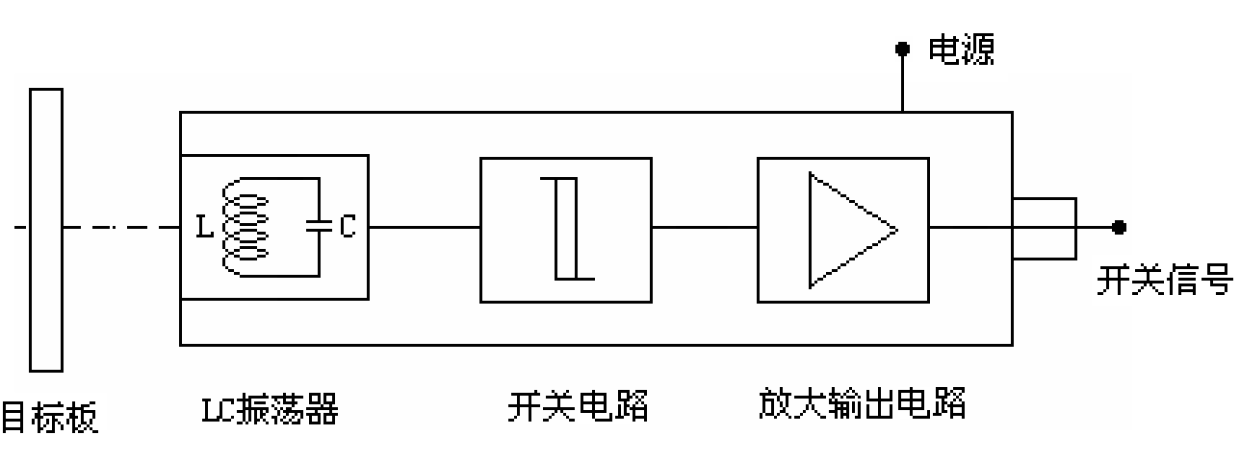
\includegraphics[width=11cm]{resource/principle.png}
	\caption{电感式传感器原理框图}
	\label{fig:sp}
	\end{figure}

	\section{实验内容与数据}
	\paragraph{电感式传感器的感应范围和回差} 本实验说明开关量传感器存在工作点和释放点。实验数据如表\ref{tab:srr}。其中,回差=(释放点-工作点)/工作点。
	\begin{table}[htbp]
		\centering
		\begin{tabular}{|c|c|c|}
			\hline
			工作点(mm) & 释放点(mm) & 回差(\%) \\
			\hline
			7.29 & 8.38 & 14.952\% \\
			\hline
		\end{tabular}
		\caption{电感式传感器的感应范围和回差}
		\label{tab:srr}
	\end{table}

	\paragraph{目标材料的宽度和厚度对电感式传感器工作点的影响}
	本实验说明目标材料的几何形状对传感器工作点的影响。实验数据如表\ref{tab:swt}。
	\begin{table}[htbp]
		\centering
		\begin{tabular}{|c|c|c|c|}
			\hline
			目标样品材料 & 工作点(mm) & 目标样品材料 & 工作点(mm) \\
			\hline
			钢板40mm宽1mm厚 &7.29 & 钢板2mm厚 5mm宽 & 5.90 \\
			钢板40mm宽3mm厚 &7.99 & 钢板2mm厚 10mm宽 & 6.51 \\
			钢板40mm宽5mm厚 &8.20 & 钢板2mm厚 18mm宽 & 7.76 \\
			\hline
		\end{tabular}
		\caption{目标材料的宽度和厚度对电感式传感器工作点的影响}
		\label{tab:swt}
	\end{table}

	\section{思考题}
	\begin{enumerate}
	\item 为什么传感器存在工作点和释放点,试从传感器的原理来分析工作点和释放点产生的原因。\\
	因为传感器为了防止在过零点产生振荡,比较器采用的是滞回比较器。由滞回比较器输入输出特性可知,其输入电压在升高、降低时跳变的临界值是不同的。因此传感器存在工作点和释放点。
	\item 目标材料的宽度和厚度对电感式传感器工作点有什么影响?为什么?\\
	由实验数据可知,当目标材料宽度一定时,工作点与材料厚度呈正相关;当目标材料厚度一定时,工作点与材料宽度呈正相关。这是因为电感式传感器依靠电磁感应在材料中制造涡流测量目标。材料宽度、厚度越大,导磁性越强,感应强度大,因此工作点远。
	\end{enumerate}

\part{磁式传感器特性研究}
	\section{工作原理}
	磁式传感器原理如图\ref{fig:ms}所示,当一个磁性目标接近传感器时,线圈铁芯的导磁性变小,线圈的电感量L也减小,而品质因素Q值增加,因而引起振荡器振荡,并使振荡电流增加,此振荡信号通过后级放大电路处理并转换成开关信号,从而达到检测物体的目的。磁式传感器可检测电磁体、永磁体或铁磁体,它的响应曲线与磁铁的位置和方向有关。
	\begin{figure}[htbp]
	\centering
	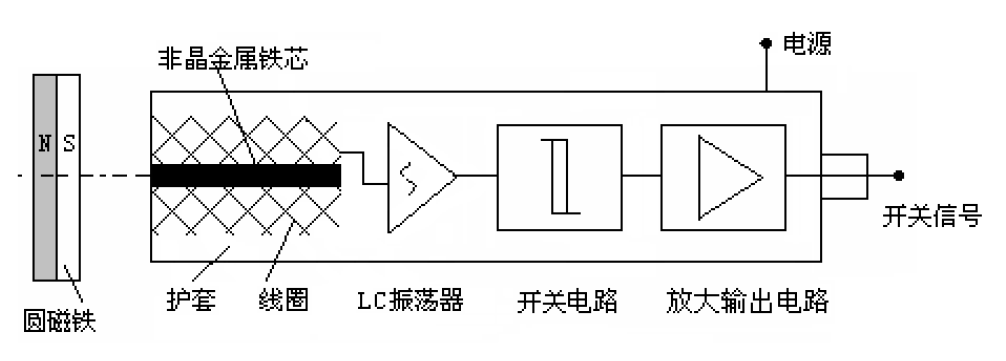
\includegraphics[width=11cm]{resource/megnet_sensor.png}
	\caption{磁式传感器原理框图}
	\label{fig:ms}
	\end{figure}

	\section{实验内容与数据}
	\paragraph{磁式传感器的感应范围和回差}
	实验数据如表\ref{tab:mrr}。由实验数据可推知,由于大磁铁磁性较大,其工作点比小磁铁更远。观察回差数据,大磁铁两种姿态的回差较为接近,而小磁铁由于工作点小,可能产生较大误差,因此不能确定回差和姿态、磁铁大小是否有关。
	\begin{table}[htbp]
		\centering
		\begin{tabular}{|c|c|c|c|}
			\hline
			目标样品材料 & 工作点(mm) & 释放点(mm) & 回差(\%) \\
			\hline
			大磁铁,平行 & 22.04 & 22.69 & 2.95\% \\
			大磁铁,垂直 & 63.64 & 65.42 & 2.80\% \\
			小磁铁,平行 & 8.24 & 8.79 & 6.67\% \\
			小磁铁,垂直 & 36.47 & 37.57 & 3.02\% \\
			\hline
		\end{tabular}
		\caption{磁式传感器的感应范围和回差}
		\label{tab:mrr}
	\end{table}

	\paragraph{磁式传感器的响应曲线}
	实验数据如表\ref{tab:mt}。由于实验中我们把平行、垂直理解反了,而平行状态工作点达不到50mm,因此少了一个数据。
	\begin{table}[htbp]
		\centering
		\begin{tabular}{|cc|cc|}
			\hline
			\multicolumn{4}{|c|}{大磁铁} \\
			\hline
			\multicolumn{2}{|c|}{平行} & \multicolumn{2}{|c|}{垂直} \\
			\hline
			S(mm) & X(mm) & S(mm) & X(mm) \\
			0 & 53.80 & 0 & 54.79 \\
			6 & 55.48 & 6 & 25.00 \\
			12 & 54.75 & 12 & 30.17 \\
			25 & 50.86 & 25 & 33.69 \\
			31 & 45.04 & 37 & 34.33 \\
			37 & 31.81 & 41 & 32.52 \\
			50 & N/A & & \\
			\hline
		\end{tabular}
		\caption{磁式传感器的感应范围与横向位移}
		\label{tab:mt}
	\end{table}

	感应范围和S和横向位移X的关系曲线如图\ref{fig:mr}。
	\begin{figure}[htbp]
	\centering
	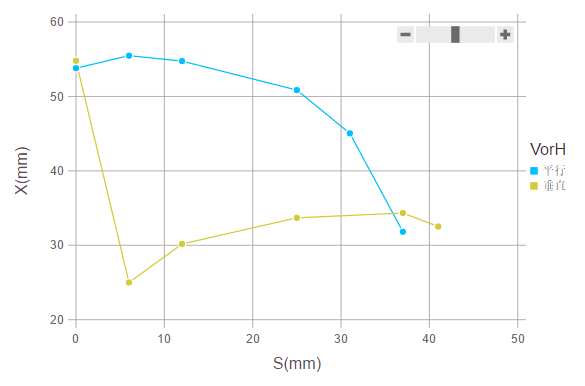
\includegraphics[width=11cm]{resource/mr.png}
	\caption{磁式传感器S-X曲线}
	\label{fig:mr}
	\end{figure}

	\section{思考题}
	\begin{enumerate}
	\item 将磁铁分别沿着垂直或平行的方向接近磁式传感器,它们的动作距离一样吗?为什么?\\
	不一样。动作距离受到磁场分布影响,工作点对应的磁感应强度大致相同。环形磁铁磁感线分布如图\ref{fig:ml}。磁铁的磁感线空间分布不均匀,水平、垂直方向也是不同的,因此动作距离呈现出不同的变化。
	\begin{figure}[htbp]
	\centering
	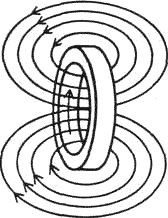
\includegraphics[width=4cm]{resource/ml.png}
	\caption{环形磁铁磁感线}
	\label{fig:ml}
	\end{figure}
	\end{enumerate}

\part{光电传感器特性研究}
	\section{工作原理}
	光电传感器一般由三部分构成,可分为发送器、接收器和检测电路。发送器对准目标发射光束,发射的光束一般来源于半导体光源、发光二极管或激光二极管。接收器由光电二极管或光电三极管组成,在接收器前面装有光学元件如透镜和光圈等,在其后面是检测电路,它能过滤掉干扰信号并输出有用信号。此外,光电传感器的结构元件中还有发射板和光导纤维(又称光纤)。
	光电传感器可分为对射型(图\ref{fig:lo})、反射板型(图\ref{fig:lr})和反射型(图\ref{fig:lb})。
	\begin{figure}[htbp]
	\begin{minipage}[t]{0.5\linewidth}
	\centering
	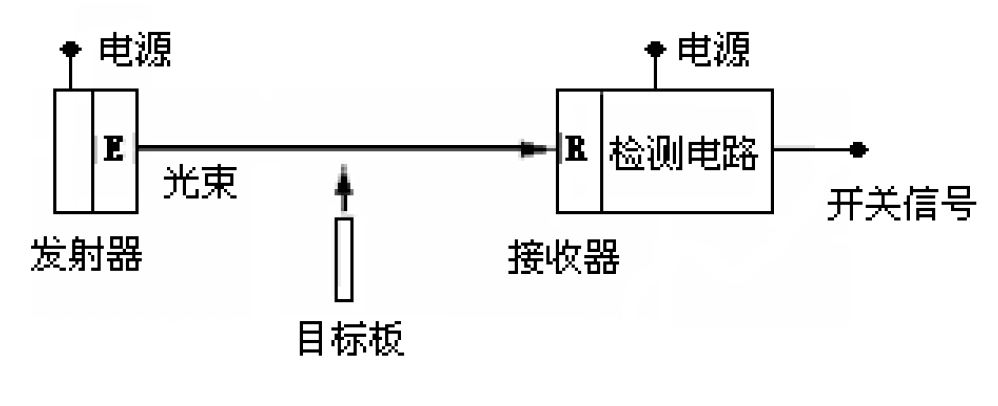
\includegraphics[width=3in]{resource/lo.png}
	\caption{对射型光电传感器}
	\label{fig:lo}
	\end{minipage}
	\begin{minipage}[t]{0.5\linewidth}
	\centering
	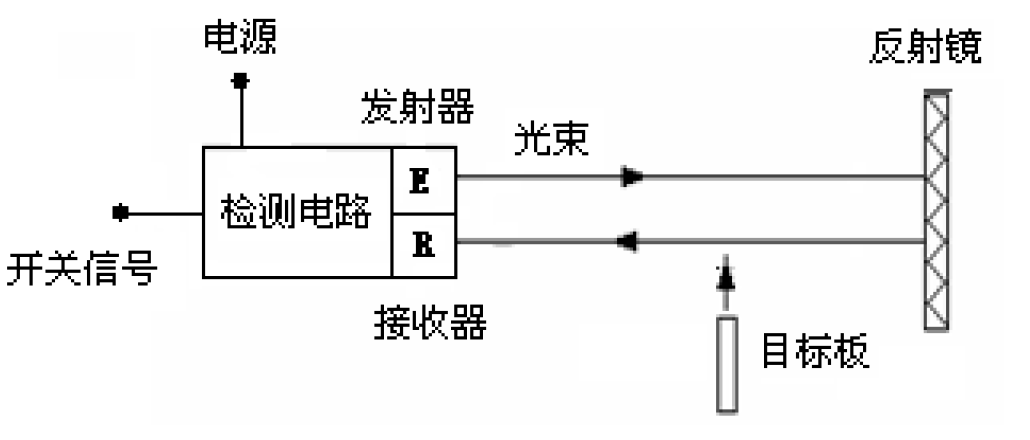
\includegraphics[width=3in]{resource/lr.png}
	\caption{反射板型光电传感器}
	\label{fig:lr}
	\end{minipage}
	\end{figure}
	\begin{figure}[htbp]
	\centering
	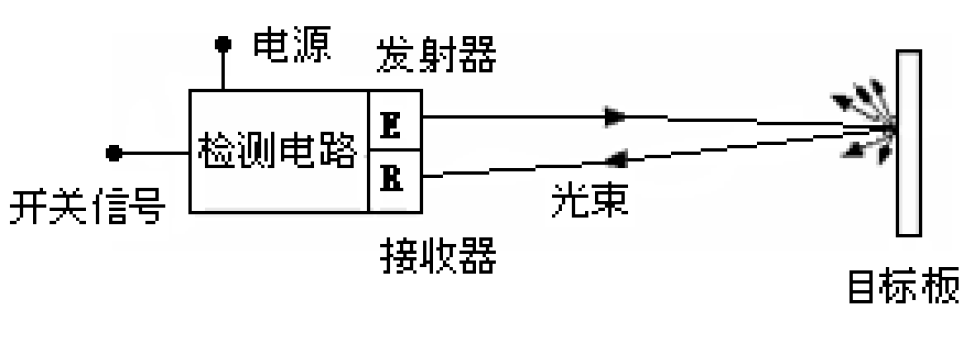
\includegraphics[width=3in]{resource/lb.png}
	\caption{反射型光电传感器}
	\label{fig:lb}
	\end{figure}

	\section{实验内容与数据}
	\paragraph{目标板的厚度对反射板型光电传感器的影响}
	实验数据如表\ref{tab:lt}
	\begin{table}[htbp]
		\centering
		\begin{tabular}{|c|c|c|}
			\hline
			目标样品材料 & \multicolumn{2}{|c|}{是否检测到目标板} \\
			\hline
			 & 是 & 否 \\
			 \hline
			白色塑料片40mm宽1mm厚 & \checkmark & \quad \\
			红色塑料片40mm宽2mm厚 & \checkmark & \quad \\
			白色塑料片40mm宽4mm厚 & \checkmark & \quad \\
			白色塑料片40mm宽6mm厚 & \checkmark & \quad \\
			白色塑料片40mm宽10mm厚 & \checkmark & \quad \\
			\hline
		\end{tabular}
		\caption{目标板厚度对反射板型光电传感器的影响}
		\label{tab:lt}
	\end{table}

	\paragraph{带光导杆的光电传感器的衰减系数}
	实验数据如表\ref{tab:ls}。其中工作点$S=S_v-S_a$,衰减系数$R=S/S_{white}$。
	\begin{table}[htbp]
		\centering
		\begin{tabular}{|c|c|c|c|c|}
			\hline
			目标样品材料 & 开关量位移 $S_v$(mm) & 标尺示数 $S_a$(mm) & 工作点 $S$(mm) & 衰减系数 $R$(\%) \\
			\hline
			标准白塑料板 & 50 & 50 & 0 & 100\% \\
			深灰色塑料板 & 50 & 11.63 & 38.37 & 76.74\% \\
			红色塑料板 & 50 & 9.43 & 40.57 & 81.14\% \\
			黑色塑料板 & 50 & 24.96 & 25.04 & 50.08\% \\
			透明塑料板 & 50 & 11.10 & 38.90 & 77.80\% \\
			半透明塑料板 & 50 & 16.62 & 33.38 & 66.76\% \\
			标准钢板ST37 & 50 & -22.20 & 72.20 & 144.4\% \\
			铜板 & 50 & -53.68 & 103.68 & 207.36\% \\
			铝板 & 50 & -50.63 & 100.63 & 201.26\% \\
			\hline
		\end{tabular}
		\caption{带光导杆的光电传感器的衰减系数}
		\label{tab:ls}
	\end{table}

	\section{思考题}
	\begin{enumerate}
	\item 说明目标板材料的厚度对光电传感器的影响。\\
	从我们的实验结果来看,无法判断目标板厚度对光电传感器是否有影响。这可能是因为实验中传感器灵敏度调的较高。
	\end{enumerate}

\part{超声波传感器特性研究实验}
\section{工作原理}
超声波传感器由超声换能器、开关电路和放大输出电路三部分组成,如图\ref{fig:sp}所示。接通电源,首先超声换能器受到激励发出超声波,然后超声波换能器转入接收状态,对收到的反射超声波进行分析。首先要确认检验到的信号是否是所发出的超声波的回声,如果检测结果是肯定的,则测量声波的行程时间,然后根据所设定的开关距离确定物体是否在开关动作范围内,如果是则激活相应的输出。\\
超声波传感器能够探测固态,液态或粉末状的物体,对于垂直于超声波传感器放置的具有光滑表面的固体及粗糙深度大于超声波波长的物体其灵敏度较高。
\begin{figure}[htbp]
\centering
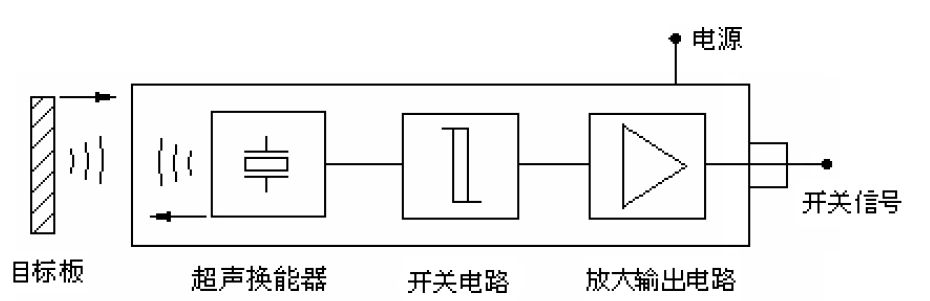
\includegraphics[width=8cm]{resource/sp.png}
\caption{超声波传感器原理框图}
\label{fig:sp}
\end{figure}

\section{实验内容与数据}
\paragraph{超声波传感器的感应范围和回差}
实验数据如表\ref{tab:lt}。由于300mm处传感器工作不稳定,往往检测不到,因此实验中将工作点A2设为225mm。另外,在实验过程中,传感器的黄灯一直在闪烁,呈现振荡的情况,而没有观察到滞回的现象,因此下面的数据都是没有意义的。
\begin{table}[htbp]
	\centering
	\begin{tabular}{|c|c||c|c|}
		\hline
		100mm处的工作点(mm) & -59.00 & 225mm处的工作点(mm) & -69.83 \\
		100mm处的释放点(mm) & -60.19 & 225mm处的释放点(mm) & -73.34 \\
		100mm处回差(\%) & 2.017\% & 300mm处回差(\%) & 5.026\% \\
		\hline
	\end{tabular}
	\caption{超声波传感器的感应范围和回差}
	\label{tab:lt}
\end{table}
\paragraph{超声波传感器的响应曲线}
实验数据如表\ref{tab:lh}。感应范围$S$与横向位移$X$图线如图\ref{fig:lsx}。由图可知,超声传感器动作距离随感应范围的增大,先增大,后减小。
\begin{table}[htbp]
	\centering
	\begin{tabular}{|c|c|}
		\hline
		传感器与目标板距离 $S$(mm) & 横向位移 $X$(mm) \\
		\hline
		60 & -56.61 \\
		100 & -63.45 \\
		150 & -67.26 \\
		200 & -72.98 \\
		250 & -76.70 \\
		275 & -75.49 \\
		300 & -70.83 \\
		\hline
	\end{tabular}
	\caption{超声波传感器的感应范围与横向位移}
	\label{tab:lh}
\end{table}

\begin{figure}[htbp]
\centering
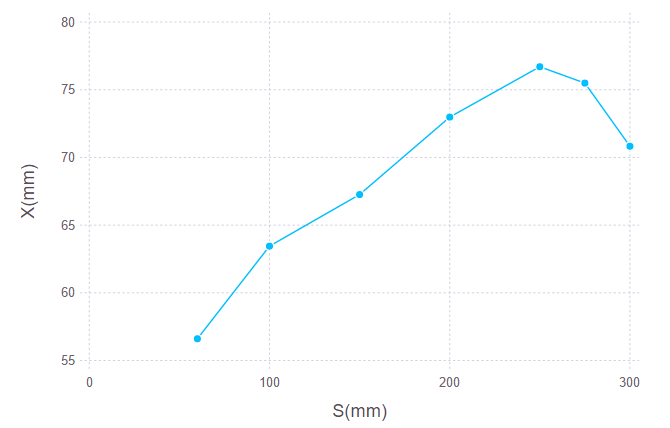
\includegraphics[width=11cm]{resource/lsx.png}
\caption{超声波传感器$S$-$X$曲线}
\label{fig:lsx}
\end{figure}

\paragraph{超声波传感器对声束偏转的检测}
本实验说明可以将声束偏转进行检测并且保持检测范围不变。

\section{思考题}
\begin{enumerate}
\item 在100mm和300mm处分别设定工作点,比较这两处的回差,解释原因。\\
由于实验中传感器黄灯在工作点附近闪烁,没有出现滞回的效应,因此不存在回差。
\item 将超声波传感器测量的两个工作点值与设定的工作点相比较,能得出什么结论?\\
\end{enumerate}

\part{模拟量传感器特性研究(电感式)}
\section{工作原理}
电感式模拟量传感器能把离金属目标的距离转变为成比例的电流输出。由于是电感式原理,所以模拟量传感器感应表面也发出一个交变的磁场,当导电的目标靠近感应面时产生涡流,损失的能量导致传感器线圈Q值下降,随着目标更接近传感器表面,使得线圈的减振更强。振荡器的特殊结构允许谐振电路的减振随距离而变化,并通过后续的电流放大器转变成近似线性的测量信号。
\section{实验内容与数据}
\paragraph{电感式模拟量传感器的输出特性}
本实验验证电感式模拟量传感器的输出电流与距离之间为线性关系。实验数据如表\ref{tab:ao},传感器传输特性曲线如图\ref{fig:af}。由传输特性曲线可知,传感器输出电流与测量距离之间基本呈线性关系,且相同电流下,目标靠近传感器过程中的距离比原理过程中的距离近,传感器略有回差。
\begin{table}[htbp]
	\centering
	\begin{tabular}{|c|c|c|c|}
		\hline
		输出电流 & 测量1组数据 & 测量2组数据 & 回差 \\
		(mA) & 距离1(mm) & 距离2(mm) & 距离2-距离1 \\
		\hline
		20.00 & -7.99 & -8.13 & 0.14 \\
		17.54 & -7.30 & -7.52 & 0.22 \\
		15.28 & -6.76 & -6.90 & 0.14 \\
		12.49 & -6.23 & -6.39 & 0.16 \\
		11.18 & -5.87 & -6.05 & 0.18 \\
		9.00 & -5.36 & -5.60 & 0.24 \\
		6.40 & -4.73 & -4.88 & 0.15 \\
		2.6 & -3.74 & -3.87 & 0.13 \\
		0.0 & -2.80 & -2.80 & 0 \\
		27.97 & -11.8 & N/A &  \\
		\hline
	\end{tabular}
	\caption{电感式模拟量传感器输出特性的测量}
	\label{tab:ao}
\end{table}

\begin{figure}[htbp]
\centering
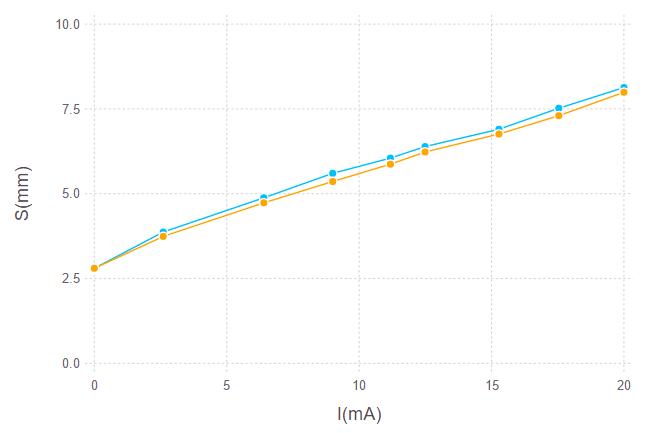
\includegraphics[width=11cm]{resource/af.png}
\caption{电感式模拟量传器输出特性曲线}
\label{fig:af}
\end{figure}

\paragraph{电感式模拟量传感器的衰减系数}
实验数据如表\ref{tab:ad}。不同材料对应标准钢板的衰减系数曲线如图\ref{fig:aff}
\begin{table}[htbp]
	\centering
	\begin{tabular}{|c|c|c|c|c|c|c|c|}
		\hline
		样品材料 & 距离1mm & 距离2mm & 距离3mm & 距离4mm & 距离6mm & 距离8mm & 距离10mm \\
		 & 电流(mA) & 电流(mA) & 电流(mA) & 电流(mA) & 电流(mA) & 电流(mA) & 电流(mA) \\
		\hline
		标准钢板 & 0.01 & 0.01 & 0.07 & 2.21 & 11.35 & 19.70 & 25.85 \\
		铜板 & 12.33 & 19.18 & 26.24 & 28.03 & 28.03 & 28.03 & 28.03 \\
		黄铜板 & 5.51 & 11.63 & 18.21 & 24.69 & 28.07 & 28.07 & 28.07 \\
		铝板 & 5.25 & 11.59 & 18.52 & 24.66 & 28.08 & 28.08 & 28.08 \\
		\hline
	\end{tabular}
	\caption{电感式模拟量传感器衰减系数的测量}
	\label{tab:ad}
\end{table}

\begin{figure}[htbp]
\centering
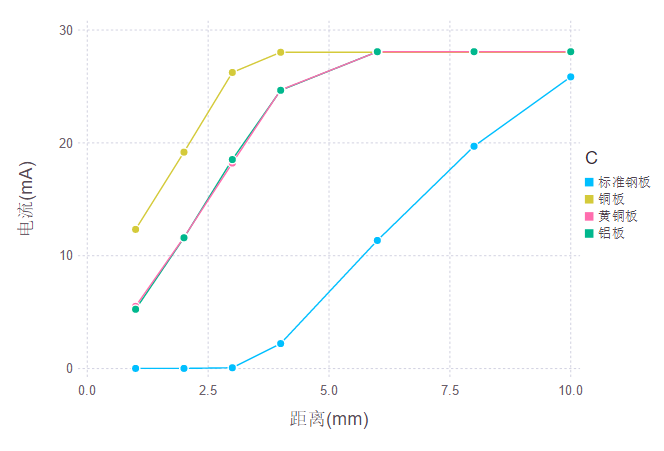
\includegraphics[width=11cm]{resource/aff.png}
\caption{不同材料对应标准钢板的衰减系数曲线}
\label{fig:aff}
\end{figure}

\paragraph{用电感式模拟量传感器测量圆孔的直径}
实验数据如表\ref{tab:ar}。从实验数据中可以看出,圆孔直径和输出电流之间并不是线性关系。这可能是由于样品材料的原因。
\begin{table}[htbp]
	\centering
	\begin{tabular}{|c|c|}
		\hline
		圆孔直径(mm) & 输出电流(mA) \\
		\hline
		6 & 7.35 \\
		12 & 6.45 \\
		18 & 9.78 \\
		\hline
	\end{tabular}
	\caption{电感式模拟量传感器圆孔直径的测量}
	\label{tab:ar}
\end{table}

\section{思考题}
\begin{enumerate}
\item 电感式模拟量传感器的测量利用的是材料的哪一个物理参量?\\
利用被测量材料的磁阻。
\item 电感式模拟量传感器可以测量圆钻孔的原理是什么?有没有可能测量更小直径?可以采取哪些方法?\\
圆孔的存在会改变产生涡流的强度,圆孔越大,涡流越小,等效于距离越远的无孔目标。为了测量更小的直径,可采用增大传感器功率、提高传感器灵敏度、调整样品位置等方法。
\end{enumerate}
\end{document}
